\documentclass[11pt,a4paper]{article}
\usepackage[margin=1.5cm]{geometry}
\usepackage[T1]{fontenc}
\usepackage[utf8]{inputenc}
\usepackage{lmodern}
\usepackage{microtype}
\usepackage{graphicx}
\usepackage{booktabs}
\usepackage{tabularx}
\usepackage{array}
\usepackage{longtable}
\usepackage{amsmath}
\usepackage{amssymb}
\usepackage{siunitx}
\usepackage{subcaption}
\usepackage{float}
\usepackage[numbers,sort&compress]{natbib}
\usepackage[colorlinks=true,linkcolor=blue,citecolor=blue,urlcolor=blue]{hyperref}
\usepackage{enumitem}

\graphicspath{{img/}}
\setlength{\parindent}{0pt}
\setlength{\parskip}{0.45em}
\setlist[itemize]{topsep=2pt,itemsep=2pt,leftmargin=1.2em}
\setlist[enumerate]{topsep=2pt,itemsep=2pt,leftmargin=1.4em}
\sisetup{
  detect-all,
  group-separator={,},
  group-minimum-digits=4,
  round-mode=places,
  round-precision=4
}

\newcommand{\repo}{\texttt{camera\_calibration\_digital\_twin}}
\newcommand{\runid}{\texttt{run\_20260406\_083611}}
\newcommand{\checkpointcommit}{\texttt{final IMU logging fix checkpoint}}

\title{\textbf{Checkpoint 01 Intermediate Report}\\[0.2em]
Camera Calibration Digital Twin}
\author{Repository-internal self-contained documentation bundle}
\date{\checkpointcommit\\Analysis run \runid}

\begin{document}
\maketitle

\begin{abstract}
This report captures the current verified state of the \repo{} repository at Checkpoint~01.
It documents the runnable browser-based simulation environment, the fiducial-tag layout, the Pixel~9a-derived camera and IMU model, the offline pose-estimation pipeline, and the numerical results attached to the preserved checkpoint analysis run \runid.
The document is meant to be sendable on its own: it includes the scene description, the relevant model parameters, representative figures copied into the report bundle, and a bibliography positioning the work relative to common camera-calibration and fiducial-tracking references such as Zhang calibration, AprilTag, IPPE-style planar pose estimation, and camera--IMU calibration pipelines \citep{zhang2000flexible,olson2011apriltag,wang2016apriltag2,collins2014ippe,furgale2013unified,rehder2017camimu}.
\end{abstract}

\section{Isaac-Oriented Simulation Environment}

\subsection{Architectural Target and Current Checkpoint Realization}

The long-term architectural target of this repository is an Isaac Sim calibration bench: a robot-mounted phone-like sensor rig moving through furnished indoor scenes, publishing camera and IMU outputs, and exposing enough ground truth to validate calibration software end to end.
The broader repo structure, API conventions, and module boundaries were designed around that target.

Checkpoint~01 does \emph{not} yet claim that the validated result set comes from a production Isaac runtime.
Instead, it preserves the first repository state where the lighter browser-based simulator already reproduces the same core experiment structure cleanly enough to be trusted as a calibration-development environment.
That distinction matters, so Table~\ref{tab:isaac-map} makes it explicit.

\begin{table}[H]
\centering
\caption{How the intended Isaac environment maps to the current checkpoint implementation.}
\label{tab:isaac-map}
\begin{tabularx}{\linewidth}{>{\raggedright\arraybackslash}p{0.28\linewidth}>{\raggedright\arraybackslash}p{0.33\linewidth}X}
\toprule
Subsystem & Isaac-oriented target & Checkpoint~01 realization \\
\midrule
World runtime & Isaac Sim scene, robot, sensors, ROS 2 bridge & browser-friendly synthetic runtime under \texttt{src/calib\_sim/interactive/} \\
Robot layer & articulated manipulator, swappable from config, Isaac articulation control & configurable kinematic arm presets with servo limits and smooth motion presets \\
Phone rig & RGB camera + IMU rigidly mounted to tool frame & Pixel~9a-style camera model + IMU profile, mounted to the synthetic end-effector \\
Scene cameras & extra fixed cameras for inspection or logging & observer-camera panels in the browser app \\
Data capture & synchronized sensor outputs and explicit ground truth & raw MP4, IMU CSV, camera truth CSV, samples JSONL, metadata JSON \\
Offline analysis & detector + calibration pipeline over recorded data & AprilTag re-detection plus JAX-based modified-Newton fitting \\
\bottomrule
\end{tabularx}
\end{table}

So when this report says ``Isaac-oriented environment,'' it means: the environment is described the way the final Isaac digital twin needs to be described, but the checkpoint metrics themselves come from the current lightweight realization that already exercises those same abstractions.

\subsection{System Role of the Environment}

The environment is not just a visual demo.
It acts as a deterministic experiment harness for calibration and pose estimation:

\begin{itemize}
  \item the robot carries a phone-like camera and IMU rig,
  \item the scene contains long-range wall tags and close-range tabletop tags,
  \item motion is repeatable and smooth enough to compare solver behavior across runs,
  \item camera ground truth, tag ground truth, and recorded outputs can be compared directly with fitted results.
\end{itemize}

That is the same role the future Isaac deployment must serve, even though the graphics and physics backend at Checkpoint~01 is lighter.

\subsection{Rendered Environment and Cameras}

Figure~\ref{fig:env-montage} shows the active checkpoint scene from the main phone view and the three observer views exposed in the web app.
This is the easiest visual summary of the environment because it immediately shows the two scale regimes that matter for the estimator: wall-mounted tags in the background and cube-top tags on the table in the foreground.

\begin{figure}[H]
  \centering
  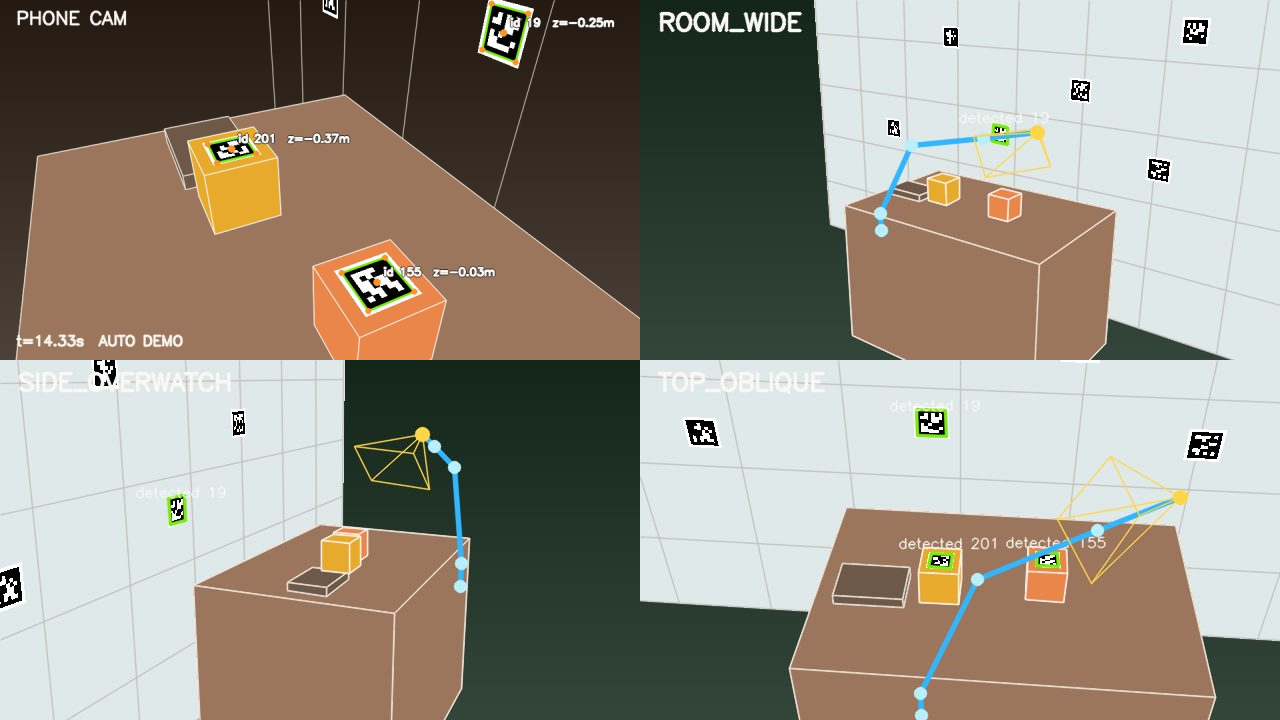
\includegraphics[width=\linewidth]{environment_montage.png}
  \caption{Current checkpoint environment rendered from the simulator.
  Top-left: primary robot-mounted phone view.
  Top-right: room-wide observer.
  Bottom-left: side observer.
  Bottom-right: top-oblique observer.}
  \label{fig:env-montage}
\end{figure}

Figure~\ref{fig:scene-topdown} complements the montage with a geometry-first top-down schematic.
It shows the backdrop wall, table, tabletop props, robot-base location, observer cameras, and the scene look-at reference used by the camera motion logic.

\begin{figure}[H]
  \centering
  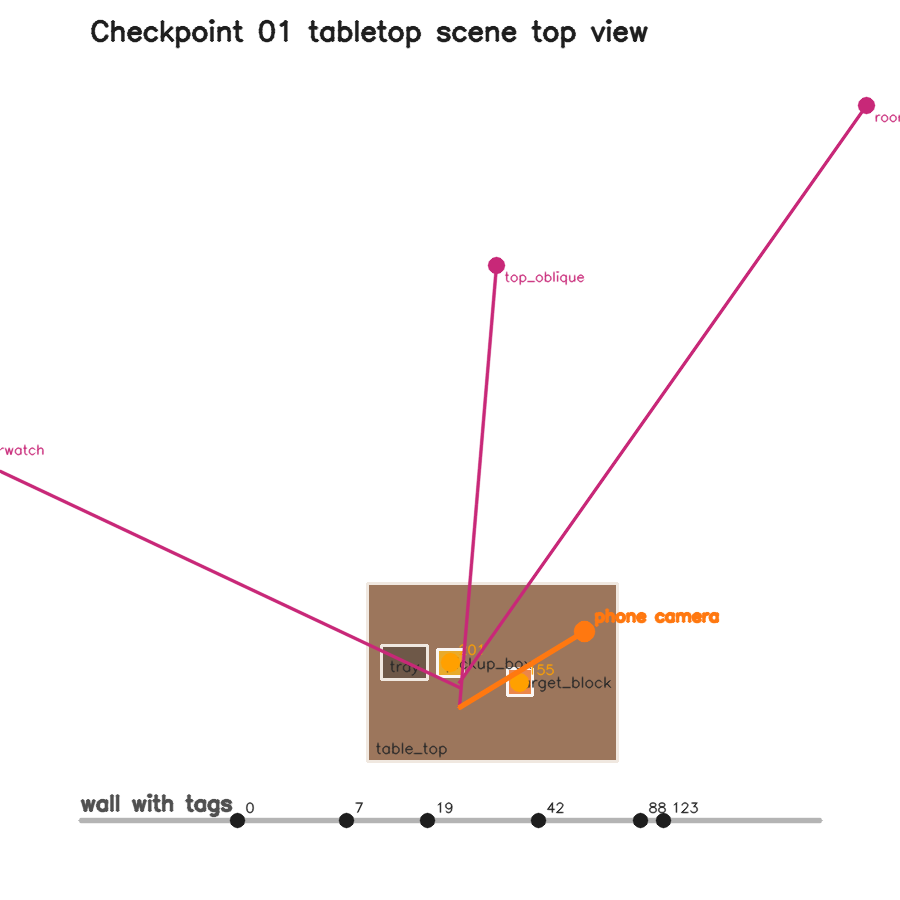
\includegraphics[width=\linewidth]{scene_topdown.png}
  \caption{Top-down schematic of the checkpoint scene.
  The wall with large tags is at $y=\SI{0.0}{\meter}$.
  The robot arm base is aligned with the table top height, allowing the phone to move around the tabletop and still look down onto the cube-top targets.}
  \label{fig:scene-topdown}
\end{figure}

\subsection{Scene Geometry}

The active environment preset is \texttt{config/interactive/tabletop\_grab\_challenge.yaml}.
It is deliberately harder than the earlier bench demo:

\begin{itemize}
  \item a large wall gives longer-range tag views and wider pose baselines,
  \item a table and props create near-field clutter,
  \item two cube-top tags introduce small targets observed at close range and from high angles,
  \item the combined layout mimics a robot trying to view or approach tabletop objects while still retaining global reference structure.
\end{itemize}

\begin{table}[H]
\centering
\caption{Scene geometry used for Checkpoint~01.}
\label{tab:scene-geometry}
\begin{tabularx}{\linewidth}{l>{\raggedright\arraybackslash}X>{\raggedright\arraybackslash}X}
\toprule
Component & Pose / size & Notes \\
\midrule
Backdrop wall & plane at $y=\SI{0.0}{\meter}$, width $\SI{3.2}{\meter}$, height $\SI{2.1}{\meter}$ & carries the larger wall-mounted tags and sets the far-reference geometry \\
Table block & center $(0.18, 0.60, 0.36)$ m, size $(1.08, 0.72, 0.72)$ m & top surface at $z=\SI{0.72}{\meter}$ \\
Target block & center $(0.30, 0.56, 0.75)$ m, size $(0.11, 0.11, 0.11)$ m & carries top-mounted tag 155 \\
Pickup box & center $(0.00, 0.64, 0.79)$ m, size $(0.11, 0.11, 0.11)$ m & carries top-mounted tag 201 \\
Tray & center $(-0.20, 0.64, 0.74)$ m, size $(0.20, 0.14, 0.03)$ m & introduces asymmetry and a manipulation-like destination prop \\
Primary scene look-at target & $(0.04, 0.46, 0.78)$ m & stabilizes the synthetic phone viewpoint across the demo motion \\
\bottomrule
\end{tabularx}
\end{table}

\subsection{Robot Arm and Motion Program}

The active arm preset is \texttt{config/interactive/robot\_arms/long\_reach\_tabletop.yaml}.
Its base position is $(0.00, 1.08, 0.72)$~m, so the base is at the same height as the table surface.
That specific choice was made to allow the camera to sweep around the tabletop rather than only look across it.

\begin{table}[H]
\centering
\caption{Robot-arm preset used at the checkpoint.}
\label{tab:robot-arm}
\begin{tabular}{lrrr}
\toprule
Parameter & Joint 1 & Joint 2 & Joint 3 \\
\midrule
Link lengths [m] & 0.34 & 0.30 & 0.22 \\
Initial servo angle [deg] & -36.0 & 60.0 & -56.0 \\
Min limit [deg] & -55.0 & -12.0 & -82.0 \\
Max limit [deg] & 55.0 & 86.0 & 76.0 \\
Speed limit [deg/s] & 66.0 & 88.0 & 108.0 \\
\bottomrule
\end{tabular}
\end{table}

The auto-demo is a smooth keyframed \SI{20}{\second} sequence.
It is not random motion: it was tuned to create repeated transitions between wall visibility, tabletop visibility, shallower views, and higher oblique views.
That makes it useful for debugging both continuity-aware initialization and multi-tag world fitting.

\begin{table}[H]
\centering
\caption{Auto-demo keyframes for the tabletop challenge.}
\label{tab:keyframes}
\begin{tabular}{rrrr}
\toprule
Time [s] & Servo 1 [deg] & Servo 2 [deg] & Servo 3 [deg] \\
\midrule
0.0 & -36.0 & 60.0 & -56.0 \\
2.4 & -20.0 & 76.0 & -78.0 \\
4.9 & -4.0 & 54.0 & -36.0 \\
7.3 & 12.0 & 70.0 & -72.0 \\
9.8 & 6.0 & 34.0 & -18.0 \\
12.6 & -16.0 & 80.0 & -80.0 \\
15.4 & -34.0 & 58.0 & -46.0 \\
17.7 & -10.0 & 66.0 & -68.0 \\
20.0 & -36.0 & 60.0 & -56.0 \\
\bottomrule
\end{tabular}
\end{table}

\subsection{Camera Views and Data Products}

The environment exposes one primary recorded phone view and three observer views.
The primary view is the only one used for the checkpoint pose-estimation results; the observer views are for operator understanding and debugging.

\begin{table}[H]
\centering
\caption{Camera views exposed by the browser app.}
\label{tab:cameras}
\begin{tabularx}{\linewidth}{lcccX}
\toprule
Camera & Resolution & Horizontal FOV & Position [m] & Purpose \\
\midrule
Primary phone view & $960 \times 540$ & $\SI{72}{\degree}$ & robot-mounted & recorded and later re-analyzed \\
Room-wide observer & $640 \times 360$ & $\SI{54}{\degree}$ & $(1.80, 2.90, 1.78)$ & whole-room debugging view \\
Side observer & $640 \times 360$ & $\SI{50}{\degree}$ & $(-2.25, 1.55, 1.42)$ & lateral visibility of arm/table geometry \\
Top-oblique observer & $640 \times 360$ & $\SI{46}{\degree}$ & $(0.20, 2.25, 2.18)$ & near top-down debugging view \\
\bottomrule
\end{tabularx}
\end{table}

Every recorded run stores both raw outputs and analysis products.
That separation is important for calibration work: raw data remain the authoritative source, while analyses can be rerun as the estimator improves.

\begin{table}[H]
\centering
\caption{Primary run artifacts stored for each recording.}
\label{tab:artifacts}
\begin{tabularx}{\linewidth}{lX}
\toprule
Artifact & Meaning \\
\midrule
\texttt{phone\_raw.mp4} & recorded primary-camera video without analysis overlays \\
\texttt{imu.csv} & synthetic accel and gyro stream in the phone IMU frame \\
\texttt{camera\_gt.csv} & camera ground-truth trajectory \\
\texttt{samples.jsonl} & per-tick state, detections, and exported measurement data \\
\texttt{metadata.json} & scene, camera, device, and run metadata \\
\texttt{analysis/report.md} & checkpoint-style markdown summary \\
\texttt{analysis/pose\_estimates.jsonl} & per-observation single-tag solves \\
\texttt{analysis/joint\_world\_estimates.jsonl} & per-frame joint world solves \\
\bottomrule
\end{tabularx}
\end{table}

\section{AprilTag Fiducial System}

\subsection{Why AprilTag is the Right Target Layer Here}

The repository uses the AprilTag \texttt{36h11} family.
This is a practical systems decision rather than a claim that no other fiducial family is viable.
The main reasons are:

\begin{itemize}
  \item AprilTag offers robust identification and low false-positive behavior for calibration-style scenes \citep{olson2011apriltag,wang2016apriltag2},
  \item square planar fiducials are convenient for controlled pose-estimation studies and compare naturally with planar-pose references such as IPPE \citep{collins2014ippe},
  \item OpenCV exposes a ready-to-run AprilTag detector path, which keeps the checkpoint easy to reproduce locally,
  \item newer work such as flexible tag layouts and low-frequency long-range tags still fits naturally into the same design space \citep{krogius2019flexible,wang2020lftag}.
\end{itemize}

Most importantly, the tags are not treated as abstract landmarks.
They are rendered into the environment, then re-detected from the recorded video.
That means the estimator sees image measurements produced by a detector, not perfect simulator correspondences.

\subsection{How the Tags are Used in This Environment}

The checkpoint environment uses two tag scales and two spatial roles:

\begin{itemize}
  \item wall-mounted \SI{0.10}{\meter} tags define the room-scale frame and produce larger pose baselines,
  \item cube-top \SI{0.06}{\meter} tags make the camera solve meaningful in the near-field tabletop task where grasp-like viewpoints dominate.
\end{itemize}

This split is deliberate.
If the scene only had far wall tags, the interesting tabletop views would not stress the estimator properly.
If it only had close tabletop tags, the system would lose long-range global reference.
Together, the tags produce a better calibration and trajectory-validation environment.

\begin{figure}[H]
  \centering
  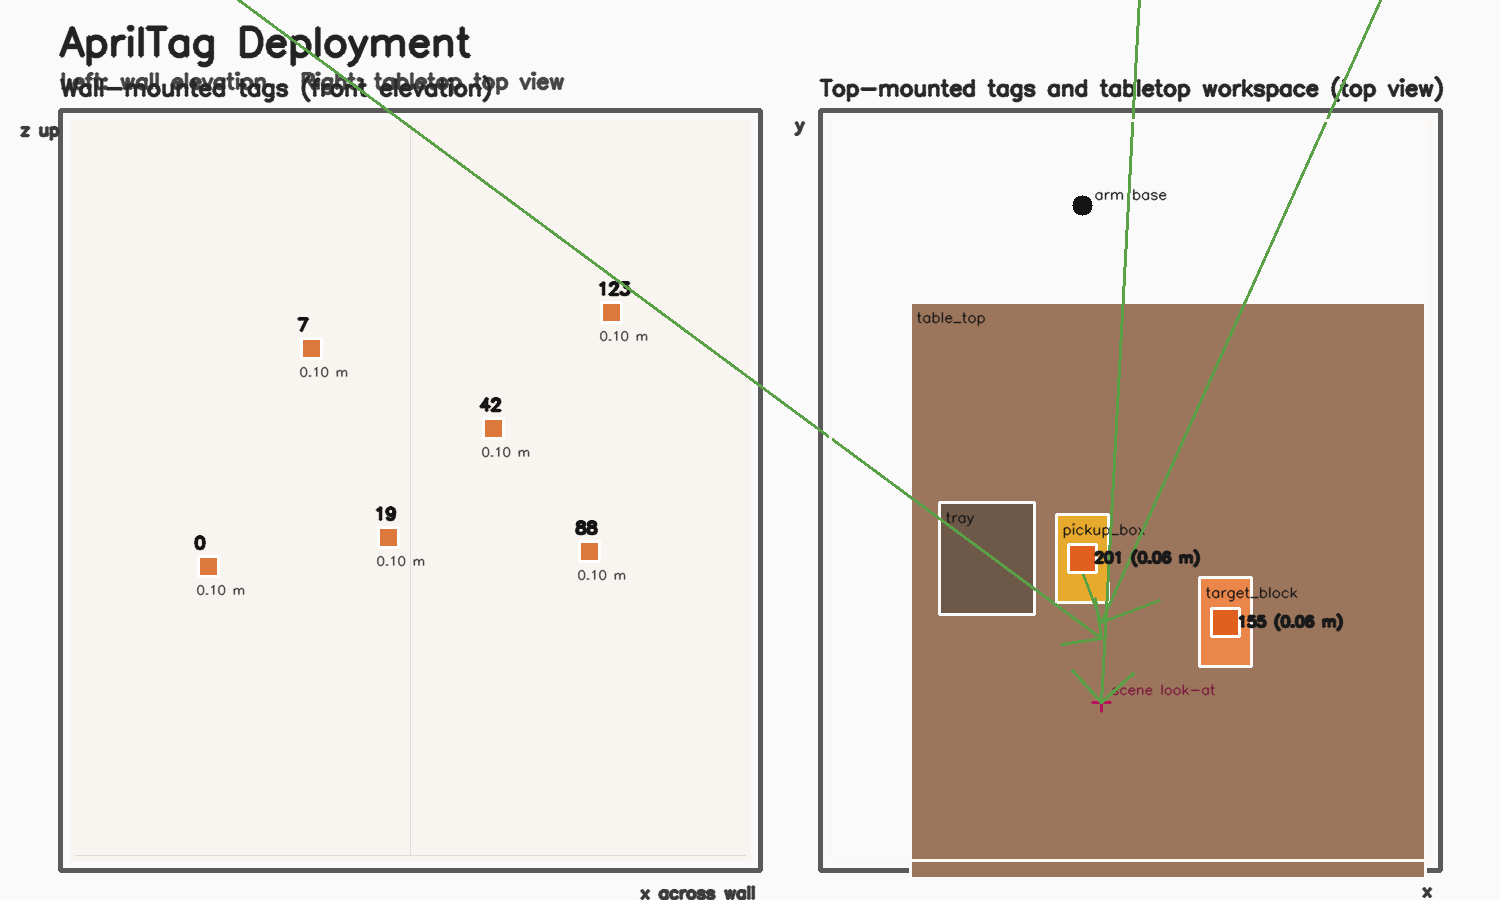
\includegraphics[width=\linewidth]{tag_layout.png}
  \caption{Configured AprilTag deployment for Checkpoint~01.
  Left: wall-mounted tags shown in wall elevation.
  Right: tabletop workspace and top-mounted tags in top view.}
  \label{fig:tag-layout}
\end{figure}

Figure~\ref{fig:phone-tag-view} shows the same idea from the primary camera itself: large wall tags remain visible as global references while the smaller cube-top tags occupy the near field during the tabletop part of the motion.

\begin{figure}[H]
  \centering
  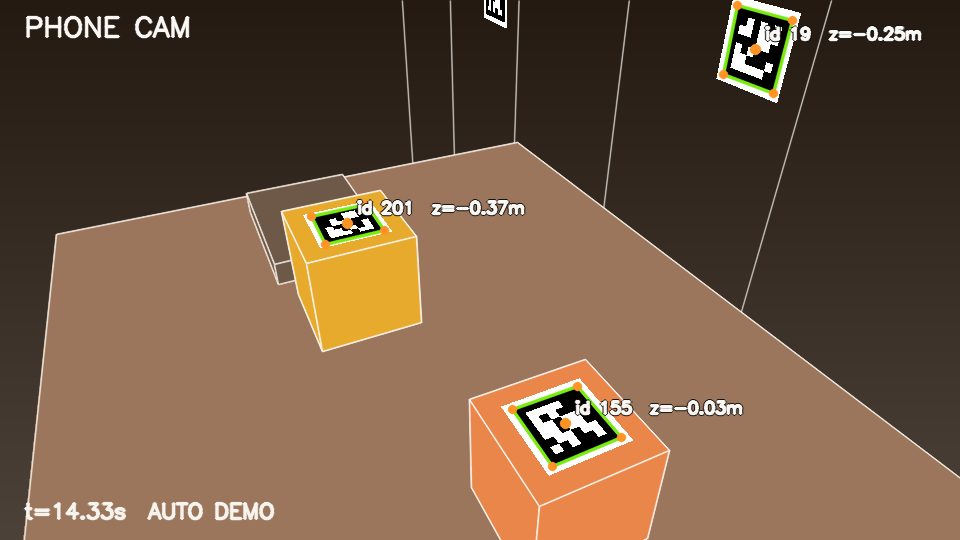
\includegraphics[width=\linewidth]{phone_view.jpg}
  \caption{Example primary-camera frame showing the mixed-scale tag regime used in the checkpoint scene.}
  \label{fig:phone-tag-view}
\end{figure}

\subsection{Configured Tag Inventory}

Table~\ref{tab:tags} lists the full configured inventory.
Only a subset is visible in every frame, which is intentional: intermittent visibility creates the track breaks needed to test continuity-aware initialization and reappearance handling.

\begin{longtable}{rcccl}
\caption{Configured fiducial tags in the checkpoint scene.}
\label{tab:tags}\\
\toprule
Tag ID & Family & Size [m] & Mount & World position [m] \\
\midrule
\endfirsthead
\toprule
Tag ID & Family & Size [m] & Mount & World position [m] \\
\midrule
\endhead
0   & 36h11 & 0.10 & wall & $(-0.92, 0.00, 0.84)$ \\
7   & 36h11 & 0.10 & wall & $(-0.45, 0.00, 1.44)$ \\
19  & 36h11 & 0.10 & wall & $(-0.10, 0.00, 0.92)$ \\
42  & 36h11 & 0.10 & wall & $( 0.38, 0.00, 1.22)$ \\
88  & 36h11 & 0.10 & wall & $( 0.82, 0.00, 0.88)$ \\
123 & 36h11 & 0.10 & wall & $( 0.92, 0.00, 1.54)$ \\
155 & 36h11 & 0.06 & top  & $( 0.30, 0.56, 0.806)$ \\
201 & 36h11 & 0.06 & top  & $( 0.00, 0.64, 0.846)$ \\
\bottomrule
\end{longtable}

\subsection{Detection Representation Used by the Solver}

The OpenCV-based detector returns four corners in clockwise order.
The repository then adds a fifth point: the projective center computed from the diagonal intersection.
The optimizer always receives the same ordered five-point observation:

\[
\left[\texttt{center}, \texttt{top\_right}, \texttt{bottom\_right}, \texttt{bottom\_left}, \texttt{top\_left}\right].
\]

This explicit ordering matters because it keeps the measurement convention stable across detector, exporter, and optimizer.
It also mirrors the local pose-estimation tooling used elsewhere in the repository.

For a tag half-extent $h$, the corresponding object points are
\[
\mathbf{P}_0=(0,0,0),\;
\mathbf{P}_1=(h,-h,0),\;
\mathbf{P}_2=(h,h,0),\;
\mathbf{P}_3=(-h,h,0),\;
\mathbf{P}_4=(-h,-h,0).
\]

\subsection{Why the Tag Section Comes Before the Camera Model}

This report now introduces the tags before the camera details on purpose.
The estimator does not operate on pixels in the abstract; it operates on image measurements of known planar objects.
So the tag geometry, size conventions, and ordering are logically prior to the camera model and the optimization method.

\section{Checkpoint Scope and Repository State}

Checkpoint~01 corresponds to commit \checkpointcommit{} and to the preserved analysis report derived from the recorded run \runid.
At this checkpoint, the repository has a clear primary path:

\begin{itemize}
  \item a browser-based interactive simulation and recording application is fully runnable,
  \item a Pixel~9a-inspired camera model is configured and verified against the recorded-phone assumptions used in this repository,
  \item raw video, IMU-like telemetry, camera ground truth, and per-frame metadata can be recorded,
  \item AprilTag-based re-detection and pose estimation can be replayed offline,
  \item continuity-aware single-tag fitting and joint all-points world-trajectory fitting are both working at checkpoint quality,
  \item the corrected recording path now preserves exact IMU/time values and exact logged start velocity well enough for effectively exact inertial dead reckoning on the preserved run.
\end{itemize}

This is intentionally not yet a full Isaac Sim production stack.
The richer Isaac/ROS runtime remains scaffold-level in the repository, while the browser simulator is the current executable reference implementation.

\subsection{Checkpoint Results at a Glance}

Table~\ref{tab:headline-metrics} summarizes the preserved metrics for the checkpoint run.
The first block is the aggregate over all single-tag solves.
The second block is the joint world-frame solve per frame, where all visible tag points are optimized together.
The third block is the corrected IMU-only dead-reckoning result after exact IMU/time persistence and exact logged initial velocity were added to the recording path.

\begin{table}[H]
\centering
\caption{Checkpoint~01 headline metrics from run \runid.}
\label{tab:headline-metrics}
\begin{tabular}{lrrr}
\toprule
Metric & Single-tag solve & Joint all-points solve & IMU-only trajectory \\
\midrule
Frames analyzed & 240 & 240 & 240 \\
Solved observations & 712 & 240 frame-level solves & 239 propagated steps \\
Mean position error [m] & 0.0042 & 0.0006 & $2.16\times10^{-7}$ \\
Median position error [m] & 0.0023 & 0.0003 & $1.43\times10^{-7}$ \\
Max position error [m] & 0.1299 & 0.0063 & $7.15\times10^{-7}$ \\
Mean rotation error [deg] & 0.2004 & 0.0806 & 0.0013 \\
Mean reprojection RMSE [px] & 0.0457 & 0.0843 & n/a \\
\bottomrule
\end{tabular}
\end{table}

The important interpretation is that the single-tag pipeline is already accurate enough for detailed per-tag analysis, the joint all-points trajectory is strong enough to serve as a trusted visual reference inside the simulator, and the corrected IMU path is now accurate enough to serve as a synthetic inertial baseline for future visual--inertial work.

\section{Camera and IMU Model}

\subsection{Source of the Phone Parameters}

Checkpoint~01 uses the preset \texttt{config/camera/pixel\_9a\_main.toml} together with the device profile \texttt{config/device/pixel\_9a\_phone.yaml}.
These values were tuned from a real Pixel~9a metadata dump collected by the companion recording workflow, then adjusted so the simulator better matches the processed MP4 output of that phone rather than an uncorrected raw sensor path.

The underlying Camera2 concepts follow the Android camera metadata definitions for lens intrinsics and distortion \citep{androidLensIntrinsics,androidLensDistortion}.

\subsection{Active-Array and Output Geometry}

The stored phone metadata describe a $4000\times3000$ active array.
The checkpoint video output is $1920\times1080$.
The repository therefore models the phone video as a center crop of the active array into a $16{:}9$ aspect ratio, followed by a scale to the output resolution.

For the active-array intrinsics $(f_x, f_y, c_x, c_y)$ and crop rectangle $(x_c, y_c, w_c, h_c)$, the effective video intrinsics are
\[
f'_x = f_x \frac{W_o}{w_c},\quad
f'_y = f_y \frac{H_o}{h_c},\quad
c'_x = (c_x - x_c)\frac{W_o}{w_c},\quad
c'_y = (c_y - y_c)\frac{H_o}{h_c}.
\]

For the current preset, the active aspect ratio is narrower than $16{:}9$, so the crop keeps the full width and trims the height.
Numerically:

\begin{itemize}
  \item active array: $4000 \times 3000$,
  \item crop rectangle: $(x_c, y_c, w_c, h_c) = (0, 375, 4000, 2250)$,
  \item output scale: $0.48$ in both axes,
  \item effective output intrinsics: $f_x=f_y=1293.17136$, $c_x=960.292272$, $c_y=543.63216$.
\end{itemize}

\begin{table}[H]
\centering
\caption{Primary phone camera parameters used for the checkpoint run.}
\label{tab:camera-model}
\begin{tabularx}{\linewidth}{l>{\raggedright\arraybackslash}X}
\toprule
Parameter group & Value \\
\midrule
Device & Google Pixel~9a, logical camera 0 \\
Sensor active array & $4000 \times 3000$ pixels \\
Output video mode & $1920 \times 1080$ pixels, center crop \\
Sensor orientation & $90^\circ$ \\
Focal length & \SI{4.53}{\milli\meter} \\
Focus distance & 0.2650956 diopters \\
Target frame rate & \SI{30}{\hertz} \\
Timestamp source & \texttt{REALTIME} \\
Active-array intrinsics & $f_x=f_y=2694.107$, $c_x=2000.6089$, $c_y=1507.567$ \\
Effective output intrinsics & $f_x=f_y=1293.17136$, $c_x=960.292272$, $c_y=543.63216$ \\
Projection preset & \texttt{pixel\_processed\_video\_default} \\
Render-time lens distortion & disabled for checkpoint~01 \\
\bottomrule
\end{tabularx}
\end{table}

\subsection{Distortion Model}

The preset keeps OpenCV Brown--Conrady coefficients
\[
[k_1, k_2, k_3, p_1, p_2] =
[0.15084998, -0.44805366, 0.38709834, 0.0, 0.0].
\]

For normalized ideal coordinates $(x, y)$ and radius $r^2=x^2+y^2$, the standard polynomial form is
\begin{align}
x_d &= x \left(1 + k_1 r^2 + k_2 r^4 + k_3 r^6\right) + 2 p_1 xy + p_2(r^2 + 2x^2), \\
y_d &= y \left(1 + k_1 r^2 + k_2 r^4 + k_3 r^6\right) + p_1(r^2 + 2y^2) + 2 p_2 xy.
\end{align}

At Checkpoint~01 these coefficients are preserved in the configuration and available to the offline analysis, but the rendered video path does \emph{not} apply additional lens warping.
This is intentional: the repository previously tested a more strongly distorted render mode and found it mismatched the actual processed-video appearance of the phone.
The checkpoint therefore models the processed MP4 path rather than a raw pre-correction sensor image.

\subsection{Image-Plane Measurement Convention}

After detection, pixel points are converted into normalized camera coordinates and then into image-plane metric coordinates using the focal length:
\[
x_m = f \frac{u-c_x}{f_x},\qquad
y_m = -f \frac{v-c_y}{f_y},
\]
where $f$ is the physical focal length in meters and $(u,v)$ are pixel coordinates.

The sign convention on $y$ makes the exported image-plane coordinates use an upward-positive axis, which matches the estimator implemented in this repository.

\subsection{IMU Model}

The checkpoint keeps a lightweight but explicit IMU profile attached to the phone.
It is not yet a full bias-random-walk inertial simulator, but after the final logging fix it is sufficient to preserve the simulator accel/gyro/time stream exactly enough for essentially exact inertial dead reckoning on the preserved checkpoint run.

\begin{table}[H]
\centering
\caption{Phone IMU parameters used by the checkpoint device preset.}
\label{tab:imu-model}
\begin{tabularx}{\linewidth}{l>{\raggedright\arraybackslash}X}
\toprule
Parameter & Value \\
\midrule
Logged checkpoint rate & \SI{12.0}{\hertz} (one sample per recorded simulation frame) \\
Gravity included & yes \\
Accel white-noise std & zero in the preserved synthetic run \\
Gyro white-noise std & zero in the preserved synthetic run \\
Accel bias & zero at checkpoint \\
Gyro bias & zero at checkpoint \\
IMU translation from camera & $(0, 0, 0.01)$ m \\
IMU orientation relative to camera & $(0, 0, 0)^\circ$ \\
\bottomrule
\end{tabularx}
\end{table}

\section{Offline Analysis and Pose Fitting}

\subsection{Pipeline Overview}

The checkpoint analysis replays the recorded run offline and performs the following steps:

\begin{enumerate}
  \item load the run metadata, samples, and raw phone video,
  \item choose whether the recorded image needs undistortion,
  \item run AprilTag detection on the recorded frames,
  \item export each detection into the five-point image-plane measurement vector,
  \item estimate per-tag camera pose from image measurements alone,
  \item estimate a joint world-frame camera pose from all visible tag points together,
  \item compare both families of estimates against the recorded simulator ground truth,
  \item write visual and numerical artifacts under the run's \texttt{analysis/} directory.
\end{enumerate}

\subsection{Single-Tag State and Objective}

For a single tag, the optimized state is
\[
\mathbf{x} =
\begin{bmatrix}
t_x & t_y & t_z & r_x & r_y & r_z
\end{bmatrix}^{\mathsf{T}},
\]
where $(t_x, t_y, t_z)$ is the tag-to-camera translation in meters and $(r_x, r_y, r_z)$ is a Rodrigues rotation vector.

Let $\mathbf{P}_i$ be the five object points on the tag plane and let $\hat{\mathbf{m}}_i$ be the observed image-plane points.
The prediction function is
\[
\mathbf{m}_i(\mathbf{x}) =
f
\frac{
\left(\mathbf{R}(\mathbf{r})\mathbf{P}_i + \mathbf{t}\right)_{xy}
}{
\left(\mathbf{R}(\mathbf{r})\mathbf{P}_i + \mathbf{t}\right)_{z}
}.
\]

The loss minimized by the solver is
\[
\mathcal{L}(\mathbf{x})
=
\frac{1}{2}\sum_i \left\lVert \mathbf{m}_i(\mathbf{x}) - \hat{\mathbf{m}}_i \right\rVert_2^2
+
\lambda \sum_i \min(z_i - \epsilon, 0)^2,
\]
where the second term penalizes non-positive predicted depth.

\subsection{Initialization Policy}

The checkpoint no longer uses a single global seeding rule.
Instead it uses a continuity-aware initialization policy:

\begin{itemize}
  \item the first frame of a visible tag streak uses a camera-obscura seed derived from apparent tag scale and center offset,
  \item subsequent frames in the same streak warm-start from the previous frame's solution for that same tag,
  \item if a tag reappears after disappearing, the solver can also fall back to a previous world-frame estimate from the frame-level joint fit.
\end{itemize}

This was an important checkpoint improvement: earlier versions seeded every frame from a fresh pinhole guess, which made the planar single-tag problem unnecessarily brittle.

\subsection{Modified Newton Solver}

Gradients and Hessians are computed with JAX \citep{bradbury2018jax}.
The checkpoint solver uses a modified Newton step rather than plain undamped Newton:

\[
(\mathbf{H} + \mu \mathbf{I}) \mathbf{p} = -\mathbf{g}.
\]

Here $\mathbf{g}$ is the gradient, $\mathbf{H}$ the Hessian, and $\mu$ a diagonal shift.
The solver starts from the raw Hessian step and, if the step is singular or not a descent direction, increases $\mu$ until a valid descent step is recovered.
An Armijo backtracking line search then chooses a step length $\alpha$ and updates
\[
\mathbf{x}_{k+1} = \mathbf{x}_k + \alpha \mathbf{p}_k.
\]

This specific solver choice matters because one of the main pre-checkpoint bugs was not in the camera model but in the optimization step selection: some Newton steps were being silently replaced by an almost-zero gradient fallback, which prevented motion even when the optimizer was not in a meaningful minimum.

\subsection{Joint World Solve}

In addition to per-tag solves, the pipeline performs a per-frame joint optimization over all visible points transformed into a shared world frame.
This produces a much stronger trajectory estimate and serves as the most accurate end-of-run reference in the checkpoint artifacts.

Conceptually, this is closer to a multi-target calibration observation than to a pure one-tag pose problem.
It reduces the planar ambiguity present in single-tag solves and is the main reason the joint trajectory errors are much smaller than the aggregated single-tag errors.

\subsection{Relation to Common References}

The repository's estimator is not a direct implementation of IPPE, Kalibr, or any single canonical package.
Instead it is a project-specific optimizer informed by those lines of work:

\begin{itemize}
  \item Zhang calibration gives the standard planar-camera-calibration background \citep{zhang2000flexible},
  \item IPPE is a strong reference point for planar-pose ambiguity and efficiency \citep{collins2014ippe},
  \item camera--IMU calibration pipelines such as Kalibr motivate the broader structure of synchronized camera and inertial metadata in a calibration system \citep{furgale2013unified,rehder2017camimu},
  \item JAX supplies the practical automatic-differentiation machinery for gradients and Hessians \citep{bradbury2018jax}.
\end{itemize}

\section{Checkpoint 01 Results}

\subsection{Per-Tag Summary}

Only four configured tags contribute heavily to the checkpoint metrics because they dominate the visible portions of the motion.
Table~\ref{tab:per-tag-results} lists the verified per-tag statistics from the preserved run.

\begin{table}[H]
\centering
\caption{Per-tag pose-estimation results at Checkpoint~01.}
\label{tab:per-tag-results}
\begin{tabular}{rrrrrrr}
\toprule
Tag & Obs. & Mean pos. [m] & Median pos. [m] & Max pos. [m] & Mean rot. [deg] & Mean reproj. [px] \\
\midrule
0   & 95  & 0.0095 & 0.0090 & 0.0211 & 0.3069 & 0.0628 \\
19  & 180 & 0.0066 & 0.0033 & 0.1299 & 0.3044 & 0.0594 \\
155 & 240 & 0.0016 & 0.0013 & 0.0102 & 0.1272 & 0.0333 \\
201 & 197 & 0.0025 & 0.0021 & 0.0090 & 0.1434 & 0.0401 \\
\bottomrule
\end{tabular}
\end{table}

The best overall per-tag behavior comes from the tabletop cube-top tags (155 and 201), which are closer to the camera and usually occupy a larger portion of the image.
Tag~19 is the only tag with a clearly visible tail in the maximum position error, reaching \SI{0.1299}{\meter} on its worst observation; this is still below the earlier meter-scale failures seen before the solver corrections.

\subsection{Representative Diagnostic Views}

Figure~\ref{fig:representative-fit} and Figure~\ref{fig:representative-overlay} are the core checkpoint diagnostics copied from the preserved run.
They show that the checkpoint is not only numerically good on average but also visually self-consistent in a representative solved frame.

\begin{figure}[H]
  \centering
  \begin{subfigure}[b]{\linewidth}
    \centering
    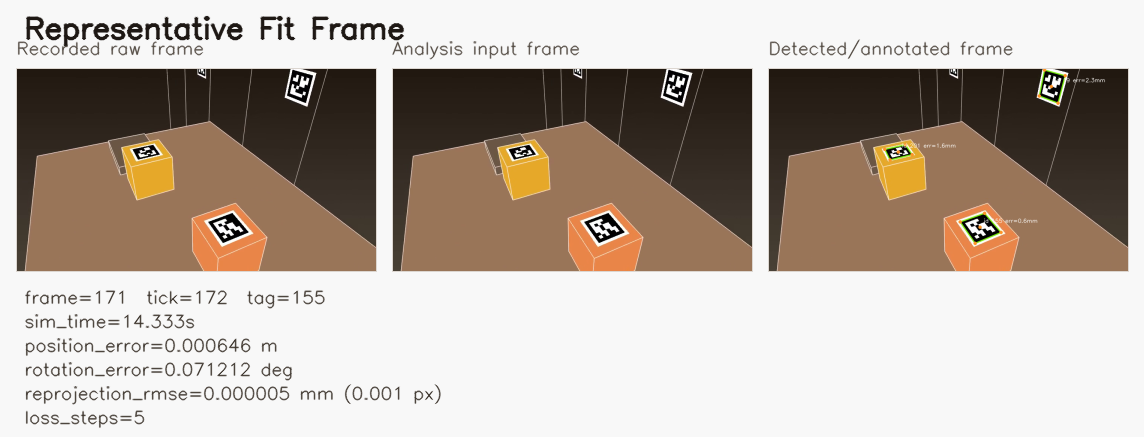
\includegraphics[width=\linewidth]{representative_fit.png}
    \caption{Representative analyzed frame.}
  \end{subfigure}
  \par\medskip
  \begin{subfigure}[b]{\linewidth}
    \centering
    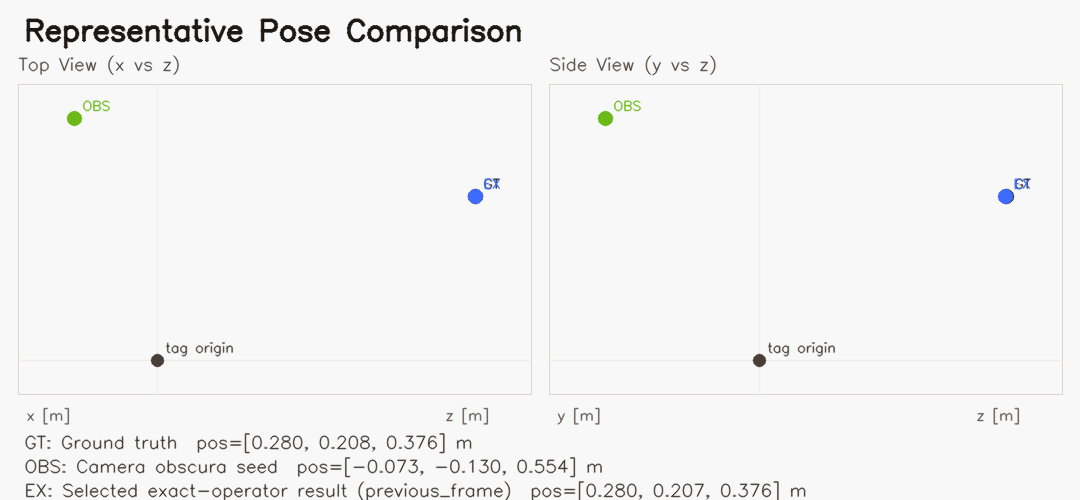
\includegraphics[width=\linewidth]{representative_pose_comparison.png}
    \caption{Ground truth and fitted camera poses for the representative observation.}
  \end{subfigure}
  \caption{Representative checkpoint diagnostics copied from the preserved run report.}
  \label{fig:representative-fit}
\end{figure}

\begin{figure}[H]
  \centering
  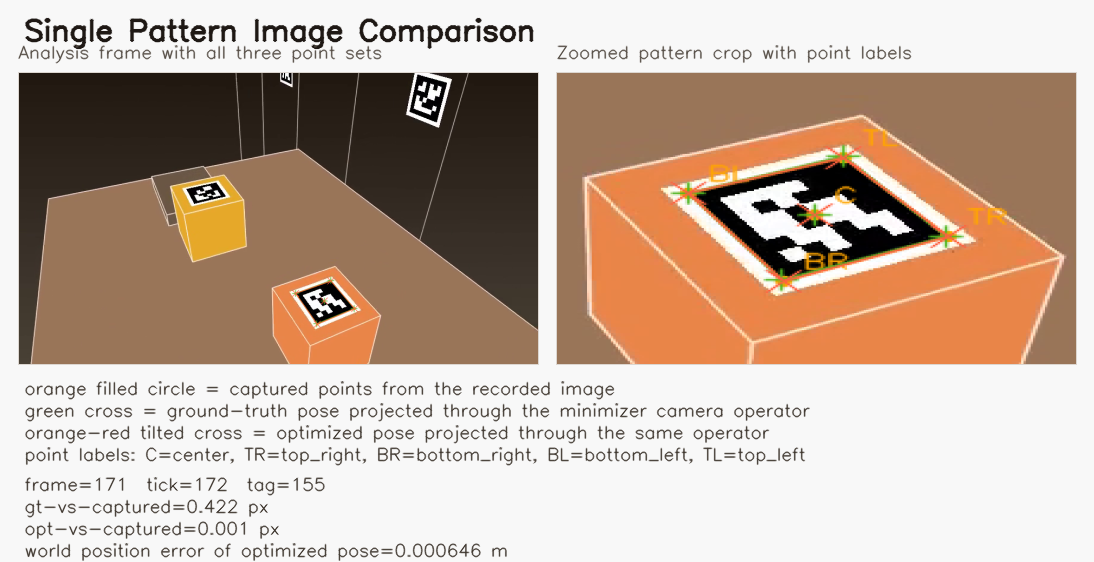
\includegraphics[width=\linewidth]{single_pattern_overlay.png}
  \caption{Representative single-pattern overlay.
  Orange circles are detected image points, green marks show the camera operator at ground truth, and orange-red tilted crosses show the final fitted result.}
  \label{fig:representative-overlay}
\end{figure}

\subsection{Global Error Timelines}

Figure~\ref{fig:global-errors} shows the two key scalar diagnostics:

\begin{itemize}
  \item world-space camera-position error in meters,
  \item image-space reprojection RMSE in pixels.
\end{itemize}

The difference between these units matters.
Small reprojection error does not automatically imply small world-space error in a planar single-tag problem, but by Checkpoint~01 both have been brought into a plausible regime.

\begin{figure}[H]
  \centering
  \begin{subfigure}[b]{\linewidth}
    \centering
    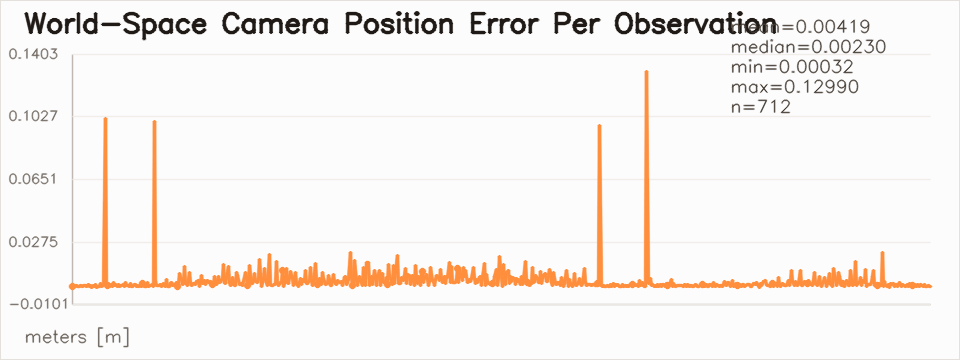
\includegraphics[width=\linewidth]{position_error_timeline.png}
    \caption{World-space camera-position error [m].}
  \end{subfigure}
  \par\medskip
  \begin{subfigure}[b]{\linewidth}
    \centering
    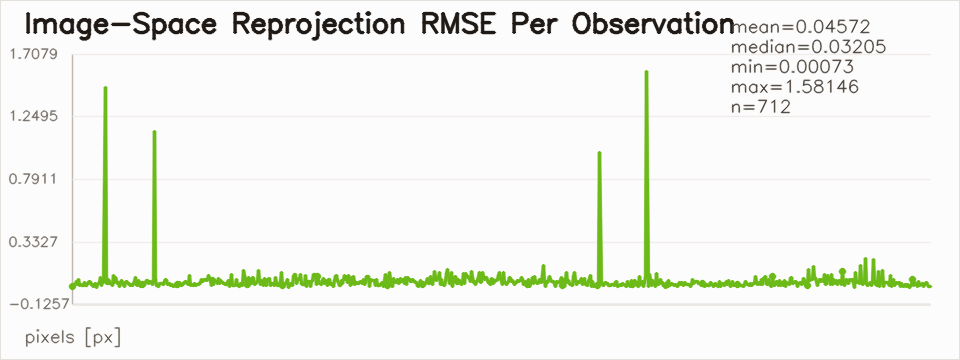
\includegraphics[width=\linewidth]{reprojection_timeline.png}
    \caption{Image-space reprojection RMSE [px].}
  \end{subfigure}
  \caption{Checkpoint-wide scalar error diagnostics.}
  \label{fig:global-errors}
\end{figure}

\subsection{Optimizer Trace}

Figure~\ref{fig:loss-trace} is the preserved representative optimizer loss trace.
It exists mainly as evidence that the corrected solver is descending as intended and no longer exhibits the broken ``no-motion'' behavior that triggered the earlier investigation cycle.

\begin{figure}[H]
  \centering
  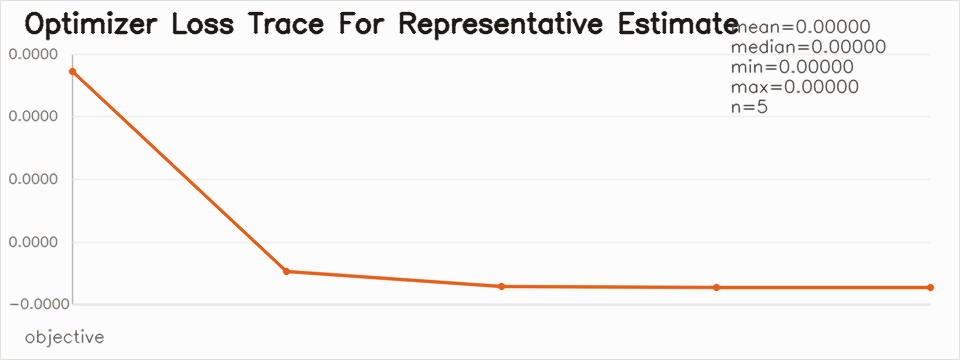
\includegraphics[width=\linewidth]{optimizer_loss_trace.png}
  \caption{Representative optimizer loss trace from the checkpoint run.}
  \label{fig:loss-trace}
\end{figure}

\subsection{World-Trajectory Comparison}

The six component plots in Figure~\ref{fig:world-pose-position} and Figure~\ref{fig:world-pose-rotation} compare, over frame index:

\begin{itemize}
  \item the independently reconstructed per-tag world-frame trajectories,
  \item the joint all-points world solution,
  \item the recorded simulator ground truth.
\end{itemize}

They are useful because they reveal consistency of the recovered trajectory, not only endpoint error statistics.

\begin{figure}[H]
  \centering
  \begin{subfigure}[b]{\linewidth}
    \centering
    
\includegraphics[width=\linewidth]{world_pose_by_tag/camera_world_x_m.png}
    \caption{$x$ [m]}
  \end{subfigure}
  \par\medskip
  \begin{subfigure}[b]{\linewidth}
    \centering
    
\includegraphics[width=\linewidth]{world_pose_by_tag/camera_world_y_m.png}
    \caption{$y$ [m]}
  \end{subfigure}
  \par\medskip
  \begin{subfigure}[b]{\linewidth}
    \centering
    
\includegraphics[width=\linewidth]{world_pose_by_tag/camera_world_z_m.png}
    \caption{$z$ [m]}
  \end{subfigure}
  \caption{World-frame position components over frame number.}
  \label{fig:world-pose-position}
\end{figure}

\begin{figure}[H]
  \centering
  \begin{subfigure}[b]{\linewidth}
    \centering
    
\includegraphics[width=\linewidth]{world_pose_by_tag/camera_world_rx_deg.png}
    \caption{$r_x$ [deg]}
  \end{subfigure}
  \par\medskip
  \begin{subfigure}[b]{\linewidth}
    \centering
    
\includegraphics[width=\linewidth]{world_pose_by_tag/camera_world_ry_deg.png}
    \caption{$r_y$ [deg]}
  \end{subfigure}
  \par\medskip
  \begin{subfigure}[b]{\linewidth}
    \centering
    
\includegraphics[width=\linewidth]{world_pose_by_tag/camera_world_rz_deg.png}
    \caption{$r_z$ [deg]}
  \end{subfigure}
  \caption{World-frame rotation components over frame number.}
  \label{fig:world-pose-rotation}
\end{figure}

\subsection{IMU-Only Trajectory Reconstruction}

The checkpoint now also includes a corrected inertial-only reconstruction driven entirely by the recorded accelerometer and gyroscope stream.
The first camera world pose is fixed to the true value, and the initial world velocity is read directly from the logged \texttt{camera\_gt.csv} trajectory.

This detail matters because the immediately preceding legacy run stored rounded IMU values and did not log the exact initial world velocity.
That older path produced visible translation drift despite the simulator being deterministic.
After fixing the recorder and matching the simulator's discrete inertial update convention in the analysis, the IMU-only trajectory became essentially exact on the preserved run.

\begin{table}[H]
\centering
\caption{IMU-only trajectory metrics from run \runid.}
\label{tab:imu-results}
\begin{tabular}{lr}
\toprule
Metric & Value \\
\midrule
Initial velocity source & \texttt{logged\_camera\_gt\_velocity} \\
Mean position error [m] & $2.1622\times10^{-7}$ \\
Median position error [m] & $1.4336\times10^{-7}$ \\
Max position error [m] & $7.1542\times10^{-7}$ \\
Mean rotation error [deg] & 0.0013 \\
Max rotation error [deg] & 0.0025 \\
\bottomrule
\end{tabular}
\end{table}

\begin{figure}[H]
  \centering
  \begin{subfigure}[b]{\linewidth}
    \centering
    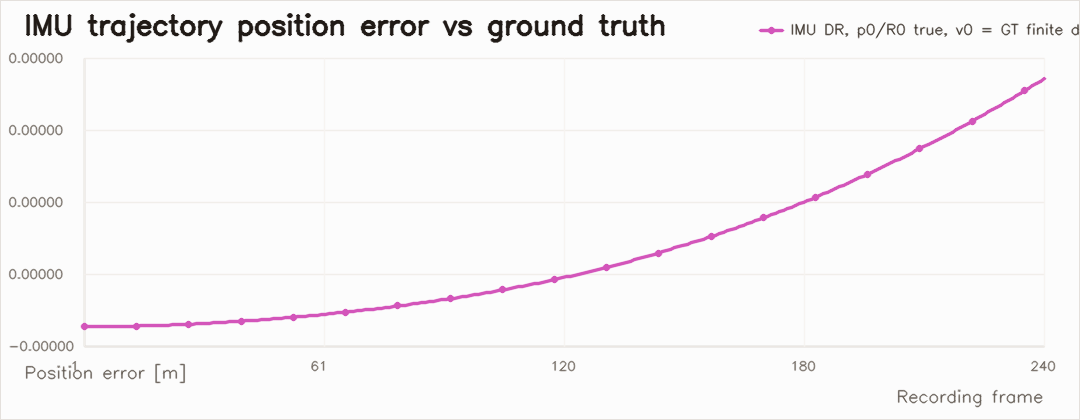
\includegraphics[width=\linewidth]{imu_position_error_timeline.png}
    \caption{IMU-only world-position error [m].}
  \end{subfigure}
  \par\medskip
  \begin{subfigure}[b]{\linewidth}
    \centering
    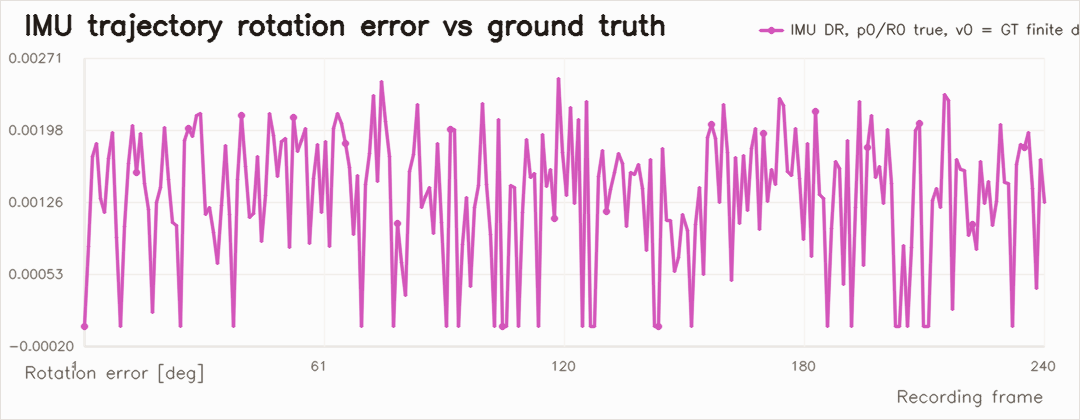
\includegraphics[width=\linewidth]{imu_rotation_error_timeline.png}
    \caption{IMU-only rotation error [deg].}
  \end{subfigure}
  \caption{Scalar IMU-only error diagnostics after the exact logging fix.}
  \label{fig:imu-errors}
\end{figure}

\begin{figure}[H]
  \centering
  \begin{subfigure}[b]{\linewidth}
    \centering
    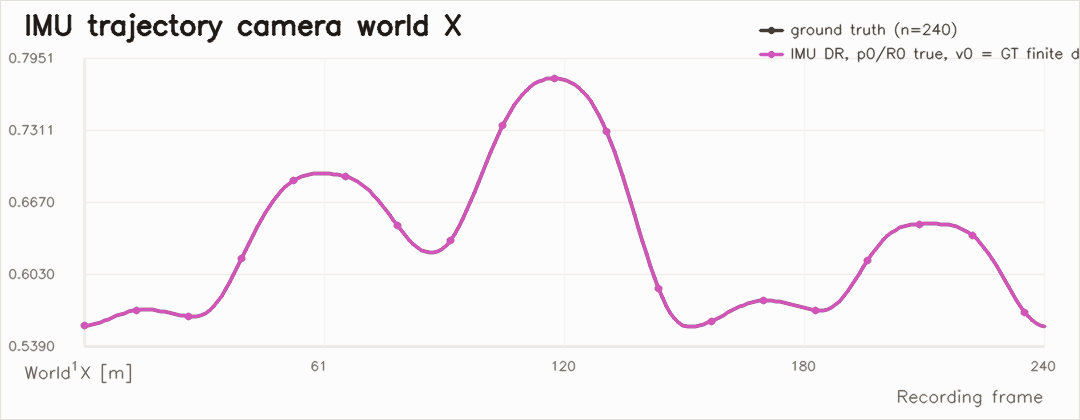
\includegraphics[width=\linewidth]{imu_world_pose/camera_world_x_m.png}
    \caption{$x$ [m]}
  \end{subfigure}
  \par\medskip
  \begin{subfigure}[b]{\linewidth}
    \centering
    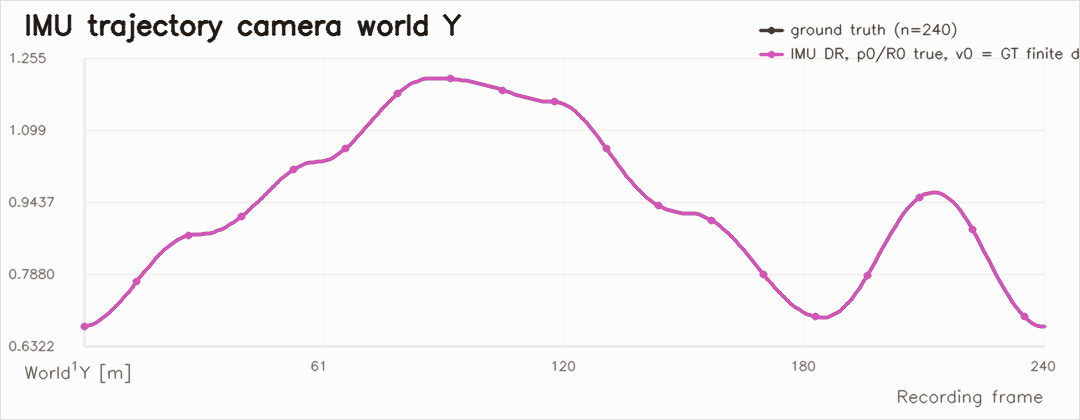
\includegraphics[width=\linewidth]{imu_world_pose/camera_world_y_m.png}
    \caption{$y$ [m]}
  \end{subfigure}
  \par\medskip
  \begin{subfigure}[b]{\linewidth}
    \centering
    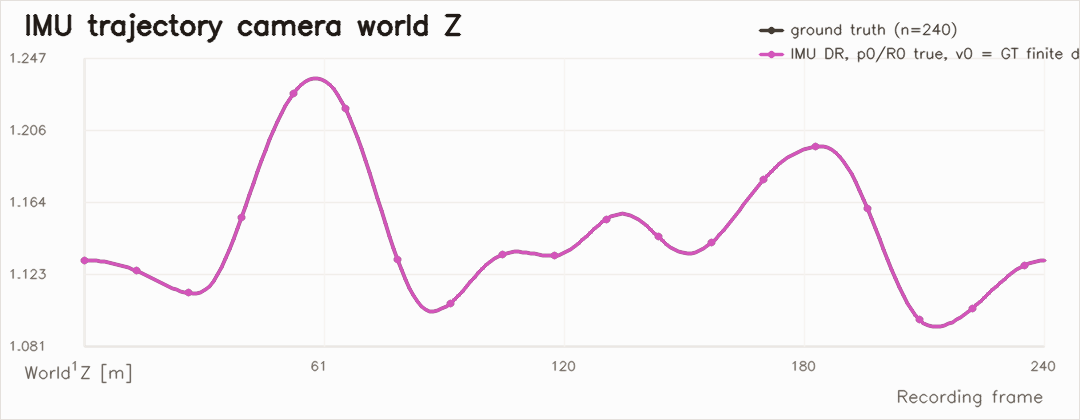
\includegraphics[width=\linewidth]{imu_world_pose/camera_world_z_m.png}
    \caption{$z$ [m]}
  \end{subfigure}
  \caption{IMU-only world-frame position components over frame number.}
  \label{fig:imu-world-position}
\end{figure}

\begin{figure}[H]
  \centering
  \begin{subfigure}[b]{\linewidth}
    \centering
    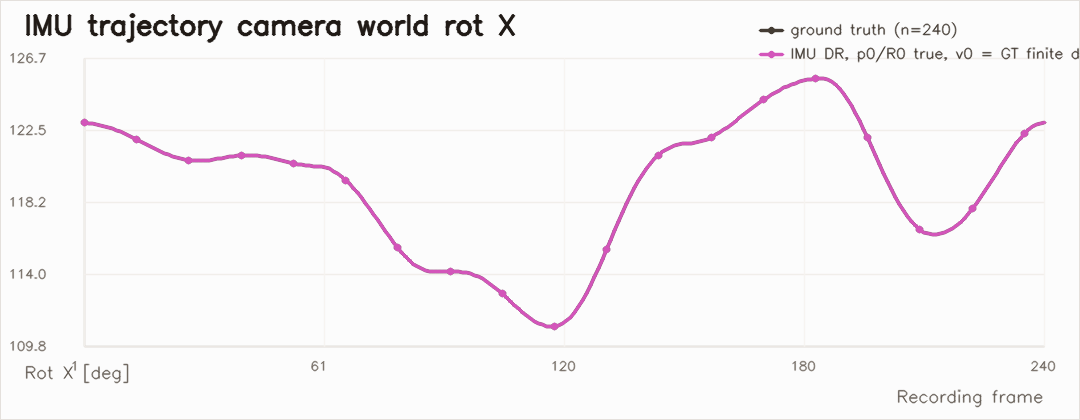
\includegraphics[width=\linewidth]{imu_world_pose/camera_world_rx_deg.png}
    \caption{$r_x$ [deg]}
  \end{subfigure}
  \par\medskip
  \begin{subfigure}[b]{\linewidth}
    \centering
    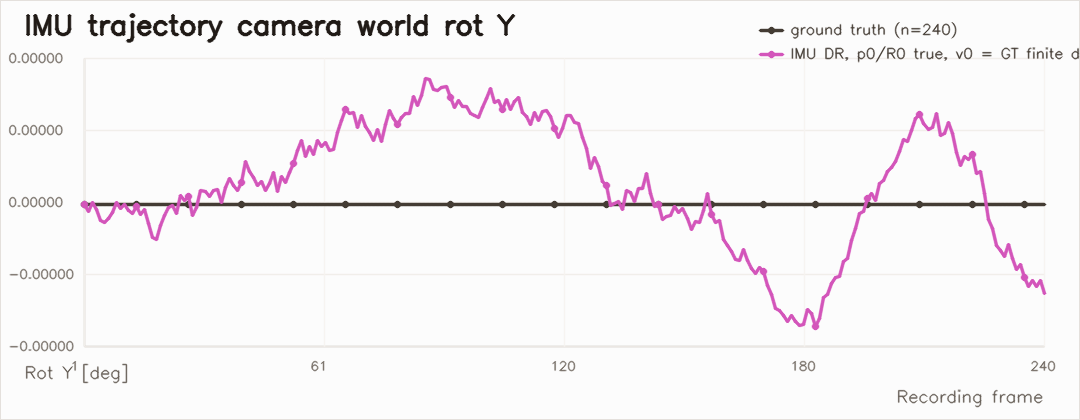
\includegraphics[width=\linewidth]{imu_world_pose/camera_world_ry_deg.png}
    \caption{$r_y$ [deg]}
  \end{subfigure}
  \par\medskip
  \begin{subfigure}[b]{\linewidth}
    \centering
    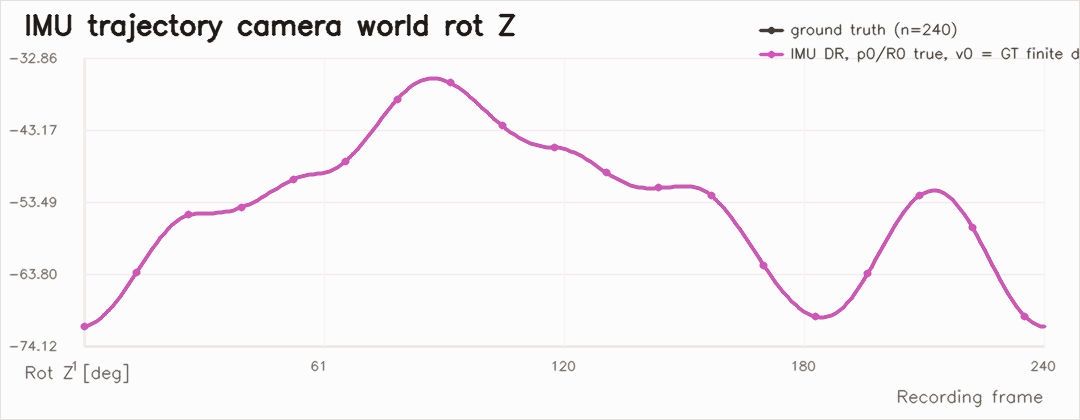
\includegraphics[width=\linewidth]{imu_world_pose/camera_world_rz_deg.png}
    \caption{$r_z$ [deg]}
  \end{subfigure}
  \caption{IMU-only world-frame rotation components over frame number.}
  \label{fig:imu-world-rotation}
\end{figure}

\subsection{Interpretation of the Checkpoint}

The current checkpoint can be summarized in three practical statements:

\begin{enumerate}
  \item The browser simulator is no longer only a qualitative demo; it now produces quantitatively useful camera-pose estimation experiments.
  \item The main failure mode discovered during development was an optimizer-step-selection bug, not a broken forward camera model.
  \item The corrected IMU recording path is now accurate enough that inertial-only trajectory reconstruction can also be used as a trustworthy synthetic reference.
\end{enumerate}

This is why Checkpoint~01 was frozen and copied into the repository documentation.
It is the first state where the app, the recorder, the camera model, the tag detector, and the offline estimator all agree well enough to preserve as a stable baseline.

\section{Limitations and Next Steps}

Even though Checkpoint~01 is strong enough to preserve, it remains a checkpoint rather than an endpoint.
The main remaining limitations are:

\begin{itemize}
  \item the simulator is still geometry-driven and browser-oriented, not a full photorealistic physics environment,
  \item the IMU model is now logged exactly enough for the preserved run, but it is still simple compared with full stochastic inertial simulation,
  \item the processed-video camera path is modeled directly, while a raw-sensor path exists only as an alternate preset,
  \item the Isaac Sim integration in the repository is still scaffold-level and not part of the validated checkpoint path.
\end{itemize}

The immediate forward path after this checkpoint is therefore not ``make the current pipeline basically work''---that part is achieved---but rather:

\begin{itemize}
  \item extend scene richness and dynamic complexity,
  \item strengthen the sensor models,
  \item connect the validated browser-side workflow to the heavier Isaac/ROS stack when that stack is ready to be real rather than aspirational.
\end{itemize}

\section{Conclusion}

Checkpoint~01 is a self-consistent, reproducible state of the repository.
It provides:

\begin{itemize}
  \item a documented synthetic scene and motion program,
  \item a concrete fiducial inventory,
  \item a Pixel~9a-derived camera and IMU model,
  \item a verified image-only pose-estimation pipeline,
  \item a verified IMU-only trajectory reconstruction path on exact persisted simulator telemetry,
  \item preserved figures and metrics that can be sent to collaborators as a stable reference.
\end{itemize}

For a project that began as a scaffold around a future digital twin, this checkpoint matters because it turns the repository into something concretely inspectable and quantitatively testable today.

\bibliographystyle{plainnat}
\bibliography{refs}

\end{document}
